\section{Monitoring und Debugging}
\label{sec:monitoring}

%TODO:\\
%- image\_publisher\\
%- image\_viewer\\
%- draw\_grid\_on\_camera\\
%- rqt\_reconfigure: (Kamera-Setup, Farbwerte, Trajektorienparameter)\\

In diesem Kapitel werden die verschiedenen Mechanismen vorgestellt, welche von uns f\"ur Monitoring und Debugging eingesetzt wurden. Ein Teil davon war hilfreich bei der Entwicklung einzelner Funktionalit\"aten, ein anderer hat die Fehlersuche im Betrieb wesentlich vereinfacht.

\subsection{image\_publisher und image\_viewer}
Mit ROS hat man die M\"oglichkeit, einzelne Nodes sehr einfach auszutauschen und somit die Funktionalit\"at schnell anzupassen, solange die Schnittstelle (die Messages) gleich bleiben. Dies haben wir uns f\"ur eine fr\"uhe Phase der Entwicklung zu Nutze gemacht. Im laufenden Betrieb liest die Bildverarbeitung Bilder aus der Webcam und ver\"offentlicht sie auf dem Topic \texttt{camera/frame}. Hierf\"ur werden aber das Fahrzeug und die dort installierte Webcam ben\"otigt.

Um auch lokal am Laptop testen zu k\"onnen, haben wir eine ROS-Node \texttt{image\_publisher} geschrieben, welche zuvor aufgenommene und lokal abgespeicherte Bilder \"offnet und published. Somit sind wir in der Lage unabh\"angig vom Fahrzeug die Bildverarbeitung zu testen und ggf. Parameter anzupassen.\\

Der umgekehrte Fall ist die Anzeige der Bilder. Im laufendem Betrieb sollten die Aufnahmen der Webcam angezeigt werden k\"onnen. Dazu wird in der ROS-Node \texttt{image\_viewer} das Topic \texttt{camera/frame} ausgelesen und das darin befindliche Bild angezeigt.
Zus\"atzlich werden die erkannten Punkte der Fahrbahnlinien sowie die daraus erzeugte 
Trajektorie aus den entprechenden Topics ausgelesen, \"uber ein 
\texttt{CameraCalibration}-Objekt zur\"uck in Bildkoordinaten transformiert und in
das angezeigte Bild eingezeichnet, wodurch eine Kontrolle der aktuell ermittelten
Linien in Echtzeit m\"oglich ist (siehe Abbildung \ref{fig:monitoring}).

\begin{figure}[!htb]
	\centering
	\begin{minipage}{.5\textwidth}
		\centering
		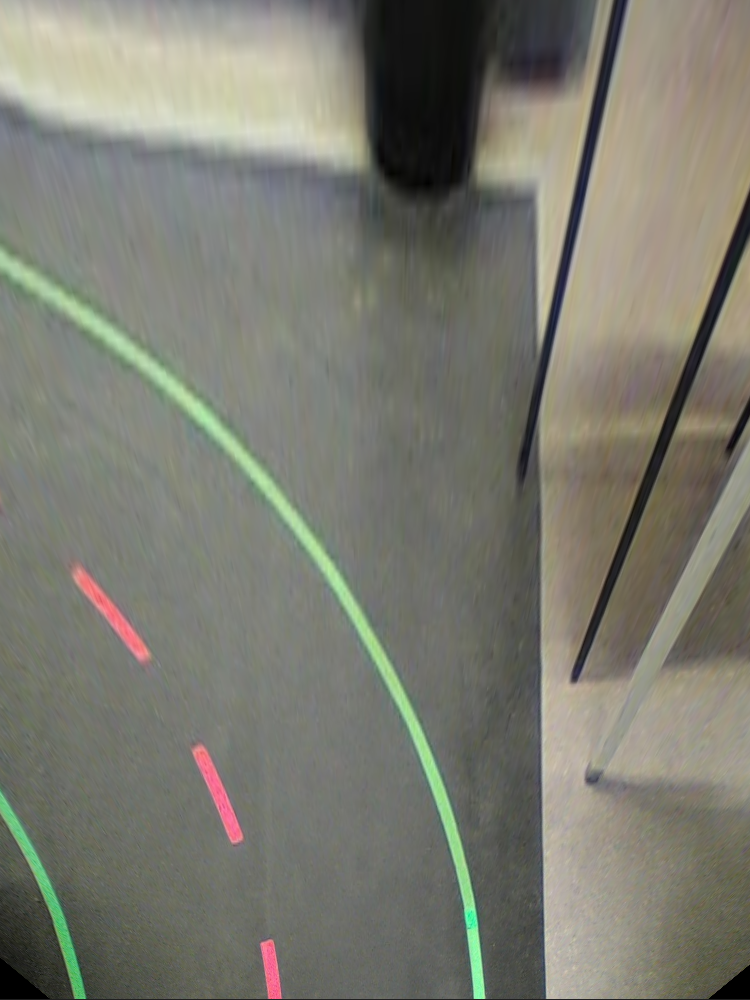
\includegraphics[width=0.7\linewidth]{images/transformed_color}
	\end{minipage}%
	\begin{minipage}{0.5\textwidth}
		\centering
		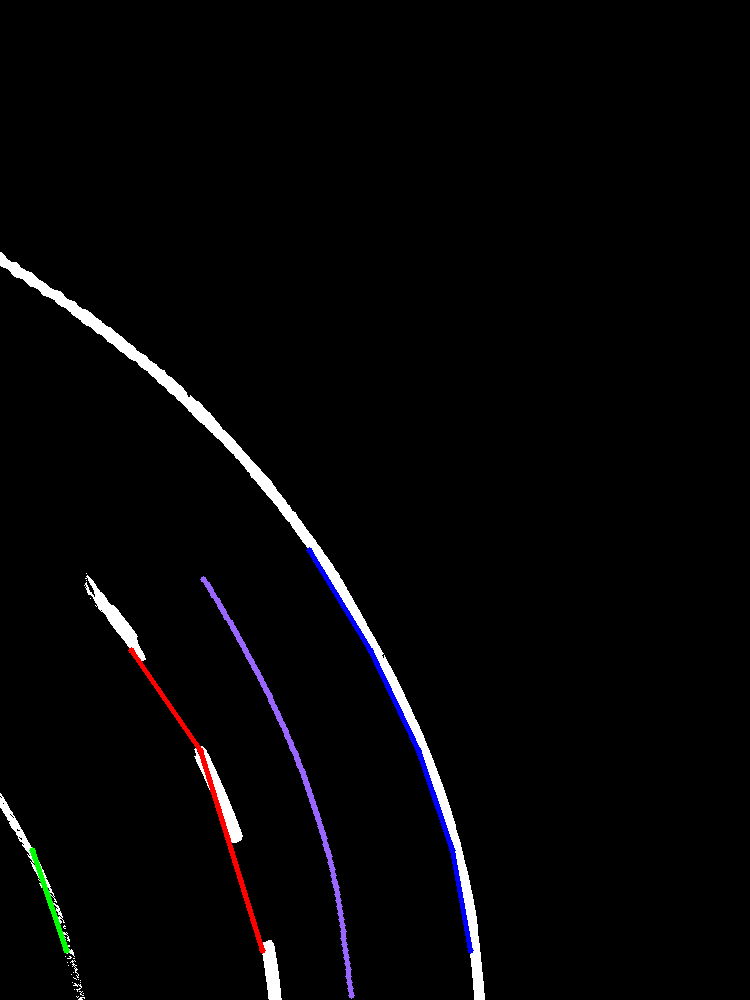
\includegraphics[width=0.7\linewidth]{images/trajectory}
	\end{minipage}
\label{fig:monitoring}
\caption{2D-Bild und zugeh\"origes Monitoring-Bild des \texttt{image\_viewer}}
\end{figure}

\subsection{Einzeichnen eines Rasters ins Bild und Aufnehmen von Fotos}
F\"ur die Transformation der Kamera-(3D-)Pixelkoordinaten in die Vogelperspektive (2D) ist wie in Abschnitt \ref{subsec:kalibrierung} beschrieben eine Kalibrierung der Kamera notwendig.
Um das hierf\"ur verwendete Referenz-Rechteck zentral im Sichtfeld der Kamera
platzieren zu k\"onnen, ist ein im Bild der Kamera eingezeichnetes Raster hilfreich.
Mangels geeigneter Webcam-Tools entschieden wir uns, eine eigene Hilfs-Node
zu implementieren, die das aktuelle Frame auf dem Topic
\texttt{camera/frame} mit Hilfe von OpenCV
zusammen mit einem Grid-Overlay anzeigt.

Sp\"ater wurde zus\"atzlich eine Funktion implementiert, um zu jeder Zeit per
Tastendruck ein Foto abspeichern zu k\"onnen, was sich zum Erstellen von Test-Bildern,
aber auch von Trainingss\"atzen f\"ur die Schildererkennung bezahlt machte.

\subsection{rqt\_reconfigure}
Da unsere Software auf dem Fahrzeug eine Viehlzahl an einzustellenden Parametern aufweist, haben wir uns f\"ur eine M\"oglichkeit zur dynamischen Rekonfiguration zur Laufzeit entschieden. Die ROS-Bibliothek bietet hier mit \textit{rqt\_reconfigure}\cite{reconfigure} einen entsprechenden Dienst an. Nachdem die zu \"andernden Parameter in einer Konfigurations-Datei vorkonfiguriert worden sind, muss man in den entsprechenden Nodes noch eine Callback Methode implementieren, welche die ge\"anderten Parameter \"ubernimmt. Somit ist man in der Lage, im laufenden Betrieb bestimmte Parameter zu ver\"andern.

Wir haben rqt\_reconfigure konkret f\"ur das Setup der Kamera (Parameter wie Helligkeit, Kontrast, ...), die Einstellung der Farbschwellwerte f\"ur die Linienerkennung (gr\"une und pinke Linie) sowie f\"ur Reglereinstellungen in der Trajektorienplanung verwendet.

\subsection{Netzwerkkommunikation}
Um die umfangreichen Optionen von Monitoring und Rekonfiguration sinnvoll nutzen zu k\"onnen, bedurfte es einer Kommunikation \"uber das Netzwerk. Da hier keine Zeitkritischen Funktionen ausgef\"uhrt werden, l\"auft die Kommunikation in unserem Projekt \"uber das Universit\"atsnetzwerk eduroam. Dazu m\"ussen das Fahrzeug, wie auch die Monitoring-Einheit, sich im Netzwerk befinden. Das Fahrzeug ist in dem Fall der ROS-Master und stellt die Daten bereit. Damit man von au\ss erhalb auf den Master zugreifen kann, muss man die IP-Adresse des Fahrzeugs wissen. Diese muss auf dem Laptop einerseits in die Datei \textbf{/etc/hosts} zusammen mit dem entsprechenden Host-Namen eingetragen sein und als Umgebungsvariable \texttt{ROS\_MASTER\_URI=http://[IP-Adresse]:11311} im Terminal exportiert werden. Danach l\"auft die Kommunikation wie gewohnt \"uber ROS.

Auf diese Weise war es uns m\"oglich, \"uber Netzwerk die Aufnahmen der Webcam an einen Monitoring-Laptop zu senden, die erkannten Linien und die geplante Trajektorie anzuzeigen und die Parameter auf dem Fahrzeug dynamisch zu rekonfigurieren. W\"ahrend unseren Versuchen hat sich eine Latenz zwischen 200 und 600ms ergeben was f\"ur unsere Monitoring und Debugging Zwecke ausreichend ist.